%
% General structure for the revdetua class:
%
\documentclass[...]{revdetua}
\usepackage{graphicx}
\usepackage{float}
\usepackage{algorithm} 
\usepackage{algorithmicx}
\usepackage{algpseudocode}
\usepackage{subfig}

\algdef{SE}[DOWHILE]{Do}{doWhile}{\algorithmicdo}[1]{\algorithmicwhile\ #1}%



%
% Valid options are:
%
%   longpaper --------- \part and \tableofcontents defined
%   shortpaper -------- \part and \tableofcontents not defined (default)
%
%   english ----------- main language is English (default)
%   portugues --------- main language is Portuguese
%
%   draft ------------- draft version
%   final ------------- final version (default)
%
%   times ------------- use times (postscript) fonts for text
%
%   mirror ------------ prints a mirror image of the paper (with dvips)
%
%   visiblelabels ----- \SL, \SN, \SP, \EL, \EN, etc. defined
%   invisiblelabels --- \SL, \SN, \SP, \EL, \EN, etc. not defined (default)
%
% Note: the final version should use the times fonts
% Note: the really final version should also use the mirror option
%

\begin{document}

\Header{1}{25}{dezembro}{2022}{0}
% Note: the month must be in Portuguese

\title{Randomized Algorithms for Combinatorial Problems}
\author{Eduardo Santos, nºmec 93107, eduardosantoshf@ua.pt} % or \author{... \and ...}
\maketitle

\begin{abstract}
The objective of this assignment was to design and test a randomized algorithm to solve the combinatorial problem from the first assignment, which was to find a minimum weighted closure for a given vertex-weighted directed graph \textit{G(V, E)}, with \textit{n} vertices and \textit{m} edges. This randomized algorithm was based on the Monte Carlo algorithms, and all the computations were made using a variety of parameters, which will be referred on the following sections.
\end{abstract}

\section{Introduction}

A randomized algorithm is an algorithm that makes use of randomly generated numbers to make decisions. This randomness is used to reduce that algorithm's time or space complexity. Monte Carlo algorithms are randomized algorithms that have, specifically in this case, a chance of not producing a solution. Let's look at the following example:
\begin{quote}
    I want to find a '0' on a binary string but only compute 5 iterations, at most.
\end{quote}

An example of a Monte Carlo algorithm to compute this problem, in pseudo-code, is:
\begin{algorithm}
\textit{i = 0}
\caption{Monte Carlo Algorithm Example} 
\begin{algorithmic}
    \Do
        \State \textit{randomly select an array element}
        \State \textit{i = i + 1}
    \doWhile{\textit{i == 5 or '0' is found}}
\end{algorithmic}
\end{algorithm}

If an '0' is found, the algorithm succeeds, if not, it fails. This algorithm will be adapted to the context of the assignment's problem and will be explained in depth later.

\section{ Problem Description}

As this assignment takes the previous one as a base, there is no need to explain again the context of finding a minimum weighted closure of a given directed graph, as it was explained previously. Given a randomly generated graph, or one read by a file, the computation of the minimum weighted closure can be very time-consuming, as the time complexity is given by:

\[
    O(2^N * N)
\]

Thus, there was a need to reduce time complexity, this can be achieved with the implementation of a randomized algorithm.
Let's consider a random graph with 5 nodes and 8 edges.

%\begin{figure}[!htb]
%    \centering
%    \includegraphics[width=0.75\columnwidth]
%{./figures/random_graph.png}
%    \caption{Example of a Random Graph}
%    \label{fig: Random Graph}
%\end{figure}

\begin{figure}[!htb]
    \centering
    \subfloat[\centering Without Solution]{{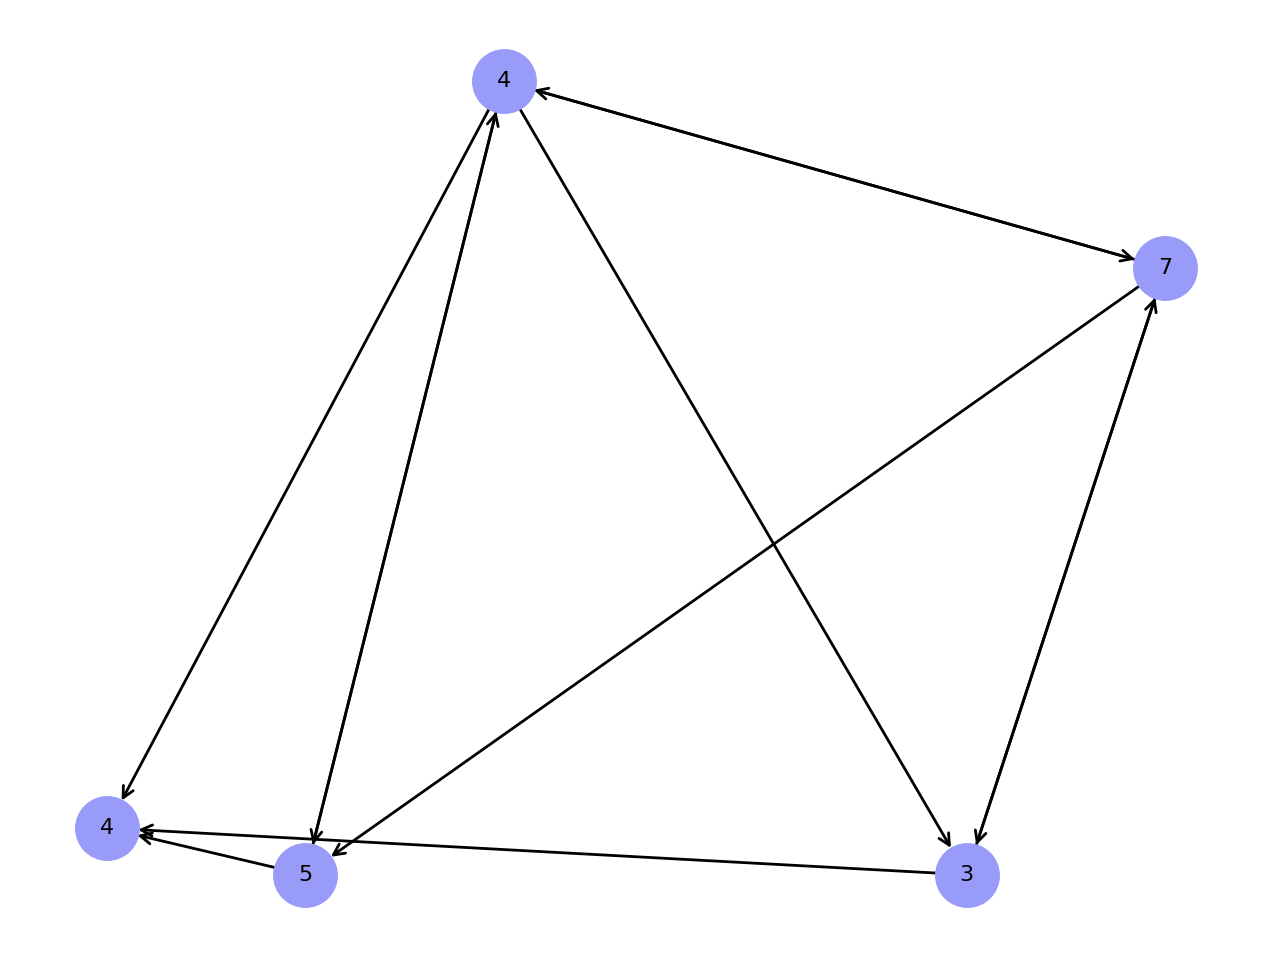
\includegraphics[width=3.65cm]{./figures/random_graph.png} }}%
    \qquad
    \subfloat[\centering With Solution]{{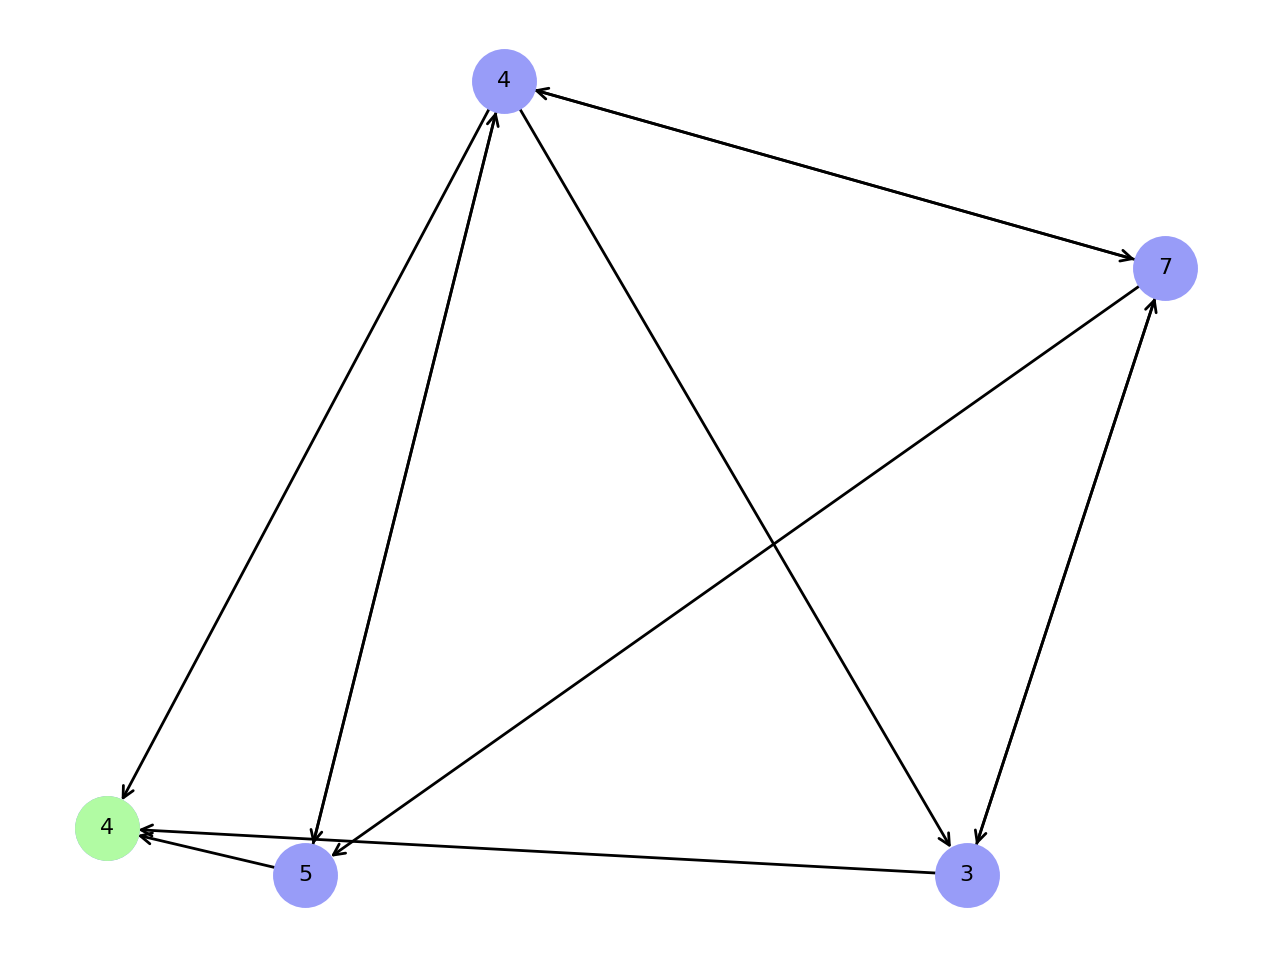
\includegraphics[width=3.65cm]{./figures/random_graph_solution.png} }}%
    \caption{Random Graph and its computed solution}%
    \label{fig:example}%
\end{figure}

% python3 main.py -r 93107 -n 5 -e 0.45

Given this example, and using the \textbf{Exhaustive Search Algorithm}, we first need to compute all the subsets (closures) of the graph, which in this case are 22, and then find the minimum weighted closure, from all candidate solutions, and that can be, as previously mentioned, very inefficient. This can be optimized by passing some parameters that control the algorithm's output. These parameters as well as the algorithm itself will be explained in the following sections.

\section{Implementation Description}

Running the main program, there are a few flags that
can be used.

\begin{figure}[!htb]
    \centering
    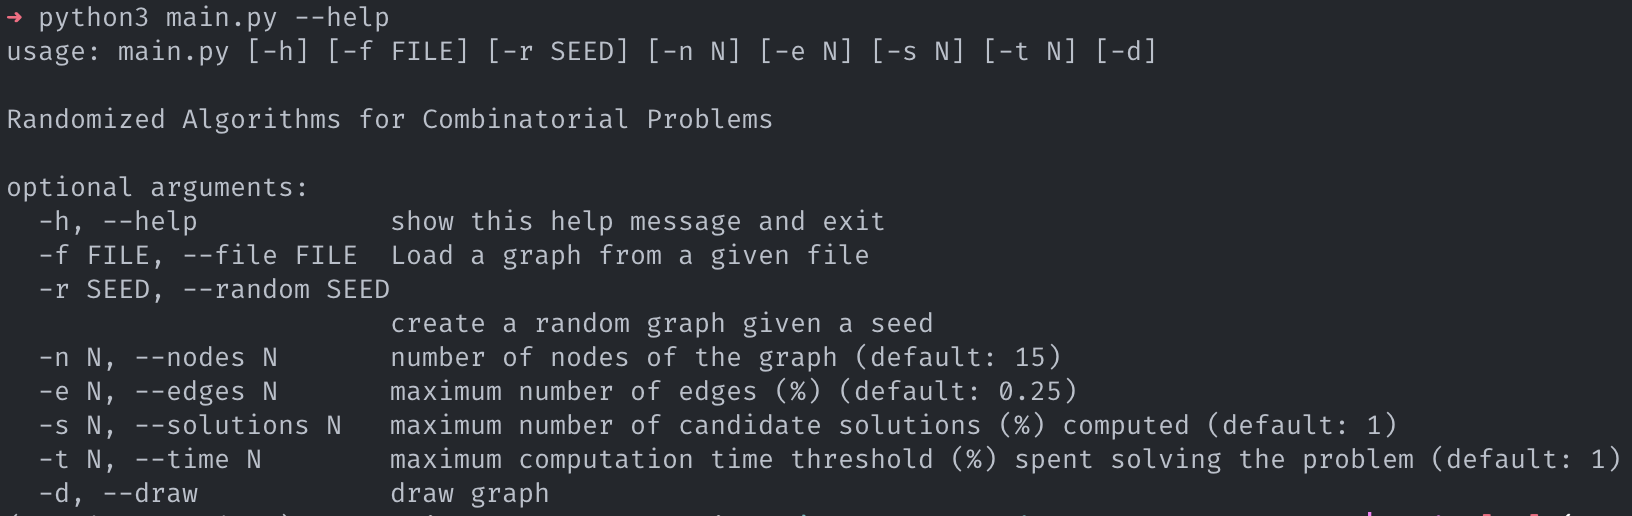
\includegraphics[width=1\columnwidth]{./figures/program_help}
    \caption{Help Menu of the Main Program}
    \label{fig: Help Menu}
\end{figure}

Most of the parameters are the same as in the previous assignment, the ones that are used as part of the randomized algorithm are:
\begin{itemize}
    \item \textbf{-s} - this flag allows the user to define the maximum number of candidate solutions to test, its value belongs in [0, 1], with 1 representing all the possible candidate solutions (100\%).
    \item \textbf{-i} - this flag allows the user to decide  when  to  stop  testing candidate solutions after spending a certain amount of computation time (in \%).
\end{itemize}

\subsection{Bug Fix}

It is important to notice that there was a bug in the previous assignment's exhaustive algorithm. Instead of only testing the subsets with edges that, in fact, existed on the graph. The algorithm computed all the combinations given the graphs' nodes and then found all the possible closures, for each combination, even if it was not present on the graph. This made the algorithm very inefficient.

On this assignment, the problem was fixed. Now, the algorithm computes only the subsets that truly exist on the given/generated graph, reducing significantly the time execution time, as well as the number of computations.

\subsection{Randomized Algorithm}

As previously mentioned, the randomized algorithm was based on the exhaustive search and on the Monte Carlo algorithms. Therefore, the algorithm decides when to stop based on a set of user-given parameters (flags), this allows for an increase in efficiency, making the solution less time and resources consuming.

As a non-deterministic algorithm, for the same input, there can be different results on each run, this gives an approximate solution, i.e., a solution that may not be the optimal one. This means that the solution computed may not be the minimum overall weighted closure, 
but instead, the relative minimum weighted closure of the computed candidate solutions.

Firstly, the algorithm computes all the subsets, \textit{S}, of the given graph. On the exhaustive search, every subset was considered a possible closure, but in this case, the \textit{sample()}\cite{random} function from the random module in Python was used to choose random subsets with the number of subsets being the maximum number of candidate solutions given by the \textbf{-s} flag. Then, for every subset, \textit{C}, it is necessary to check if there are any edges for other nodes that are not in \textit{C}. If this happens, then \textit{C} is not a closure, if not, then the subset is added to the closures list. After having all closures, every subset node’s weight is added, and the closure with the smallest sum is considered the minimum weighted closure.

Another strategy of the randomized algorithm is by using the \textbf{-t} flag. In this case, the algorithm stops computing possible closures when a certain execution time is reached, then computes the minimum weighted closure from the ones found.

Both strategies can be used simultaneously, i.e., the algorithm can stop to choose random subsets with the number of subsets being the maximum number of candidate solutions and stopping when an also given execution time is reached.

%TODO: mostrar exemplo de grafo com exhaustive vs com 50% de -s e -t

\subsubsection{Formal Computational Complexity Analysis}

Performing a formal computational analysis of the exhaustive search algorithm, regarding the time complexity, the complexity would be \textit{O(S * N * M)}, where \textit{S} is the number of subsets, \textit{N} is the number of nodes, and \textit{M} is the maximum number of edges a node can have. This is because the first \textit{for} loop iterates through the randomly chosen  subsets, \textit{S}, which is \textit{O(s)}, the second \textit{for} loop iterates through all the elements in each subset, which is \textit{O(n)}, and the third \textit{for} loop iterates through all the edges of each element in the subset, which is \textit{O(m)}. Multiplying the time complexities of the three \textit{for} loops gives the overall time complexity of the algorithm.

\begin{figure}[htp]
\centering 

\subfloat[Random Graph\label{random_graph}]{%
  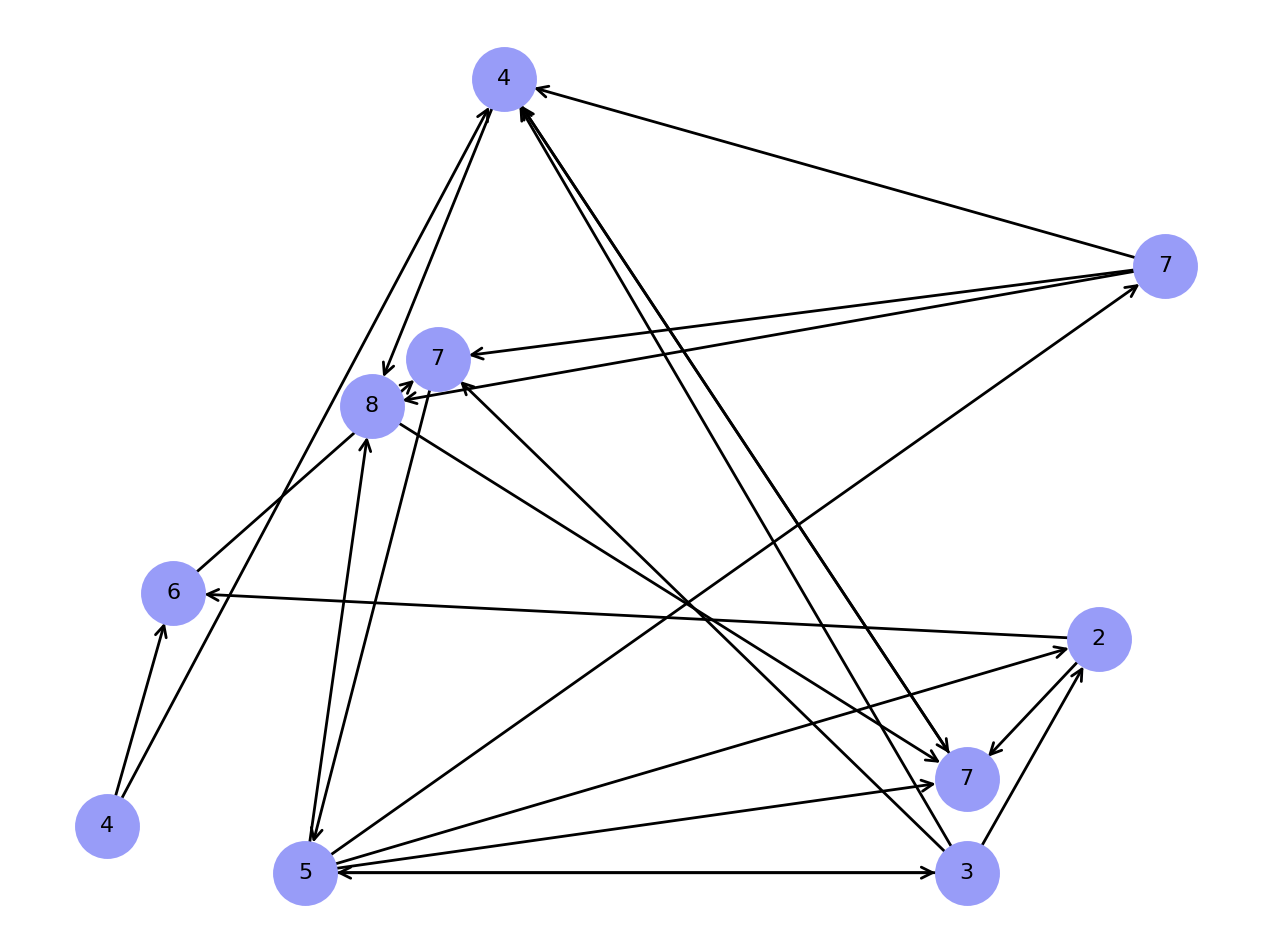
\includegraphics[clip,width=0.65\columnwidth]{figures/complex_graph.png}%
}

\subfloat[Minimum Weighted Closure Given By Exhaustive Search Algorithm\label{random_graph_exhaustive}]{%
  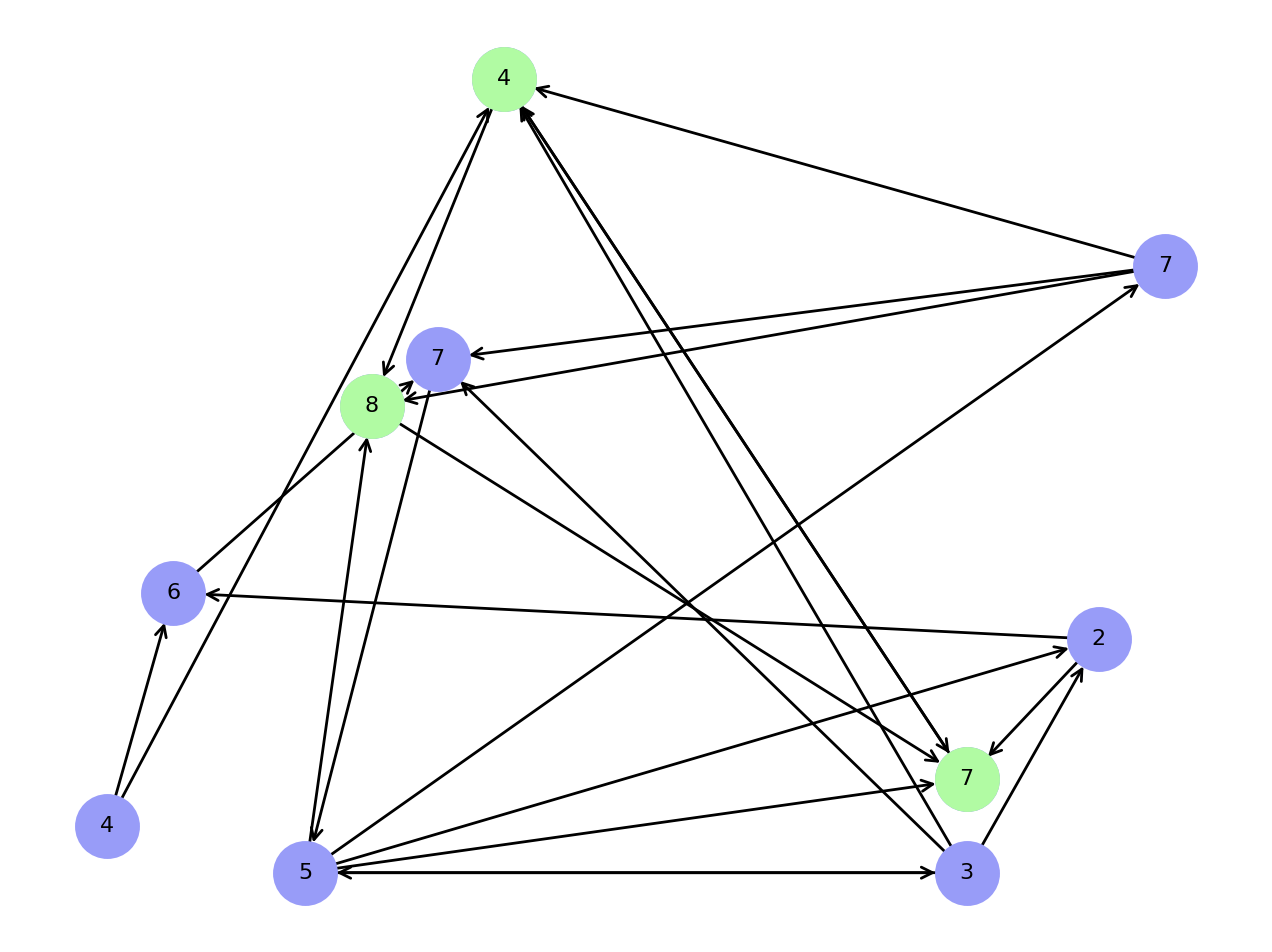
\includegraphics[clip,width=0.65\columnwidth]{figures/complex_graph_exhaustive.png}%
}

\subfloat[Minimum Weighted Closure Given By Randomized Algorithm with \textbf{-s} = 0.5\label{random_graph_randomized}]{%
  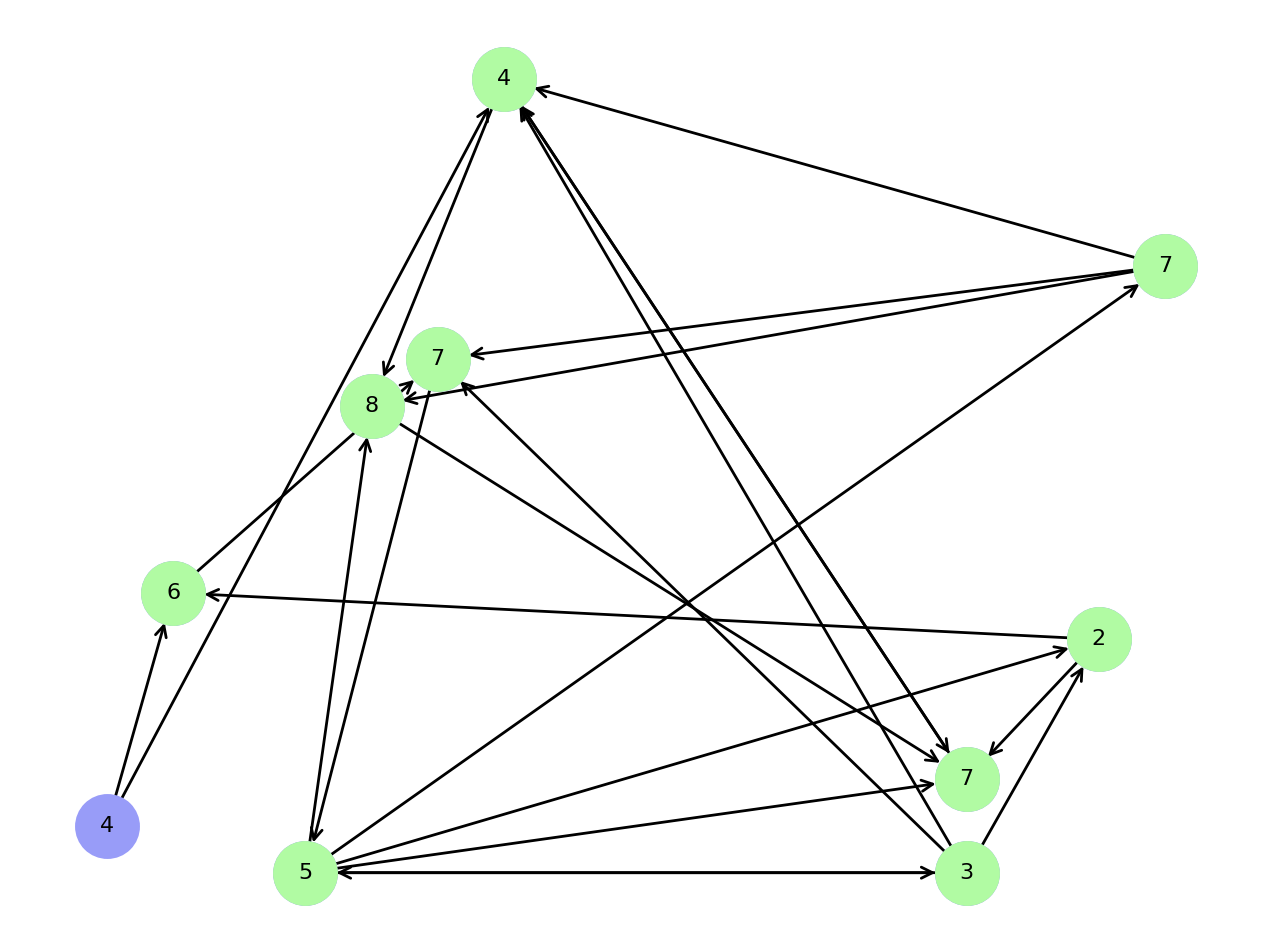
\includegraphics[clip,width=0.65\columnwidth]{figures/complex_graph_s_0.5.png}%
}

\caption{Comparison Between Exhaustive and Randomized Algorithms}

\end{figure}

In the images above there is a randomly generated graph with 11 nodes and 20\% of the maximum number of possible edges between those nodes [\ref{random_graph}]. For this graph, both exhaustive search [\ref{random_graph_exhaustive}] and randomized [\ref{random_graph_randomized}] algorithms' solutions were computed. Regarding the randomized method, the maximum number of candidate solutions given was 50\% of the maximum number of possible solutions/subsets.

The solution given by the exhaustive search is the optimal one, which means that the closure returned by the algorithm is the minimum weighted one of the whole graph subsets. As the randomized algorithm only computes half of all the possible candidate solutions, the minimum weighted closure it retrieves as a solution is, in this case, the entire graph. It is still a solution, but not the optimal one.

\section{Results and Discussion}

Several plots were drawn to better understand the difference between the randomized and the exhaustive algorithms and compare each other. Both algorithms were compared using three parameters: execution time, the number of solutions found, and the number of iterations. For each algorithm, the results were computed using successively larger random graphs with 1 to 25 nodes and 25\% of the maximum number of possible edges between nodes.
All of the results can be found in the \textbf{results/}
folder.

\begin{figure}[!htbp]
    \centering
    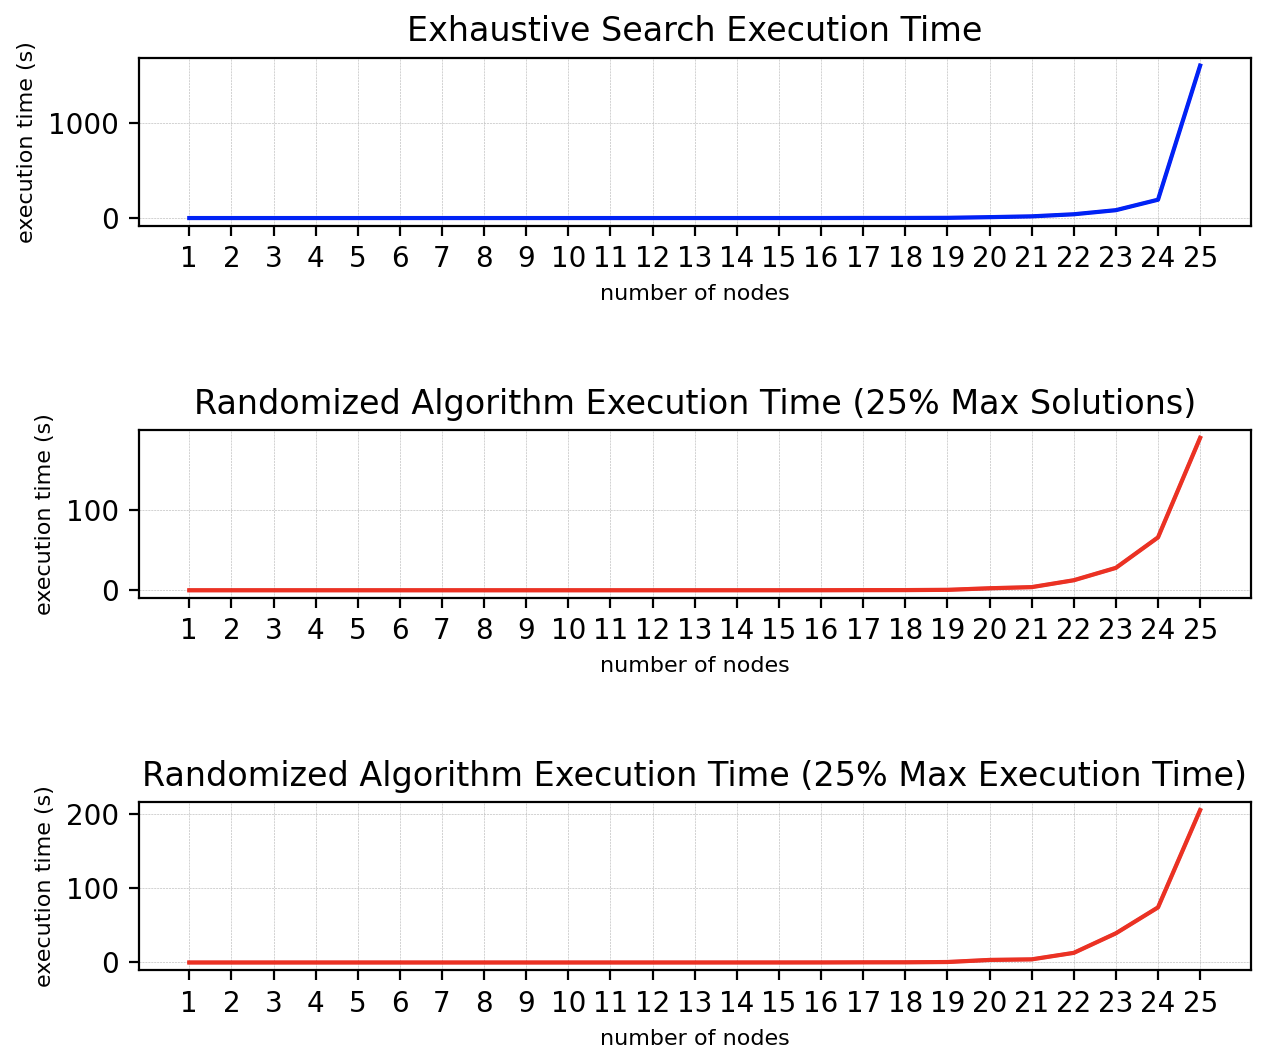
\includegraphics[width=0.9\columnwidth]{./figures/execution_time_0.25.png}
    \caption{Execution Time on the Exhaustive and Randomized Algorithms\label{execution_time}}
    \label{fig: Execution Time on the Exhaustive and Randomized Algorithms}
\end{figure}

Comparing the two algorithms, as seen in the plot [\ref{execution_time}], passing 25\% of the maximum number of candidate solutions, as well as 25\% of the maximum execution time, we get similar results between both variations of the randomized algorithm, both representing approximately 20-25\% of the previous one's execution time, when comparing to the exhaustive search. This variation is directly related to the randomly chosen subsets for the computation.

\begin{figure}[!htbp]
    \centering
    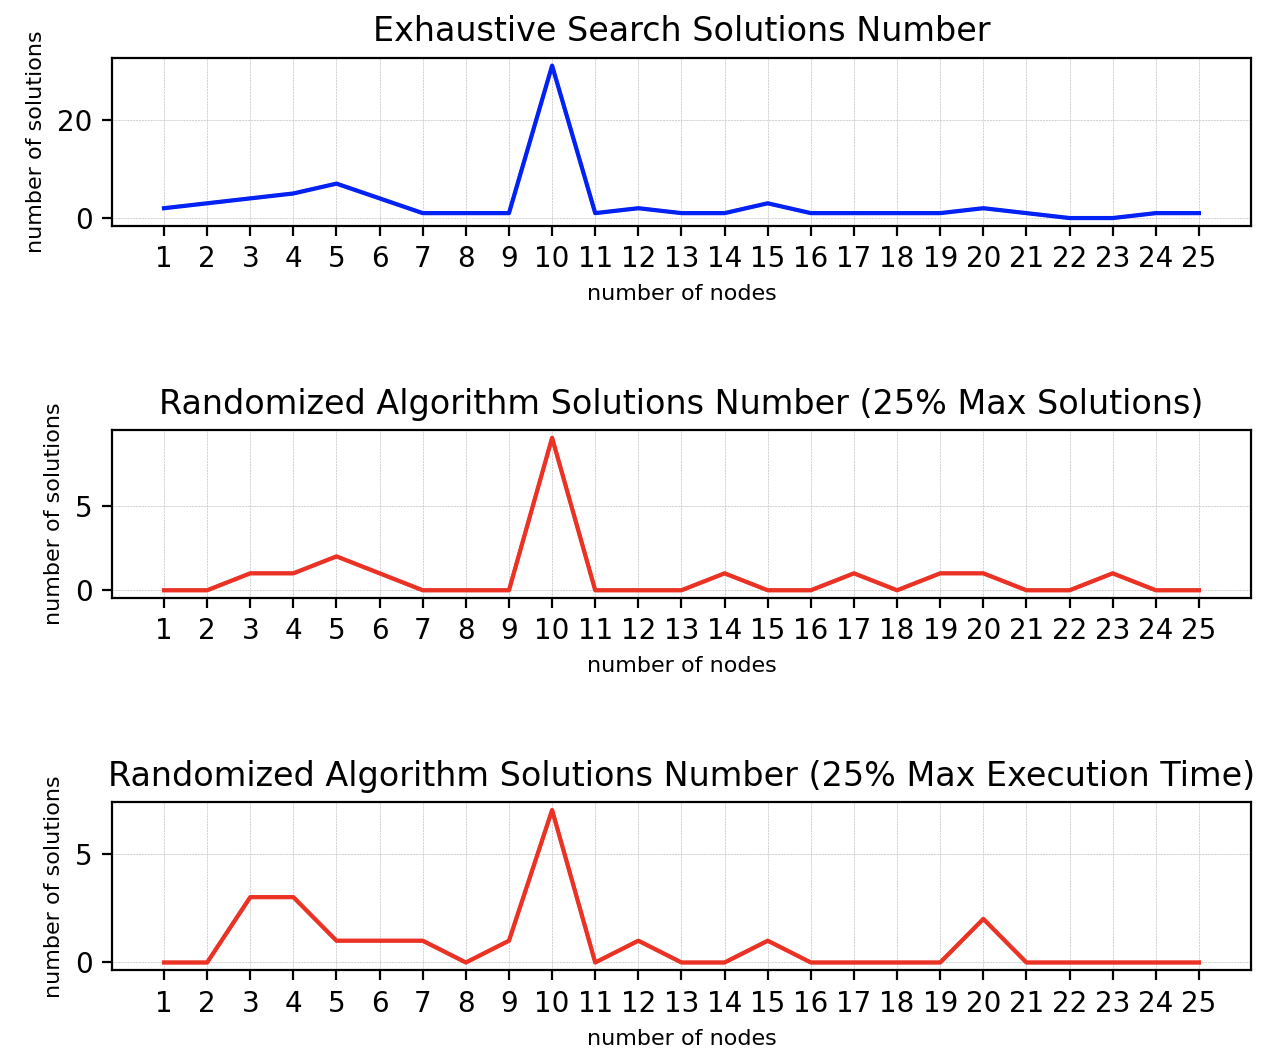
\includegraphics[width=0.9\columnwidth]{./figures/solutions_number_0.25.png}
    \caption{Solutions Number on the Exhaustive and Randomized Algorithms\label{solutions_number}}
    \label{fig: Solutions Number on the Exhaustive and Randomized Algorithms}
\end{figure}

As well as the execution time, there is also a reduction to 25\% of the solutions number [\ref{solutions_number}] of the exhaustive algorithm, both using the \textbf{-s} and \textbf{-i} parameters. It makes sense that when defining, f.e., 25\% of the maximum number of candidate solutions, the number of solutions found is approximately 25\% of the brute force solution's ones. But when passing the maximum computation time parameter, the similarity, although present, it's not as noticeable, in comparison to the \textbf{-s} flag.

\begin{figure}[!htbp]
    \centering
    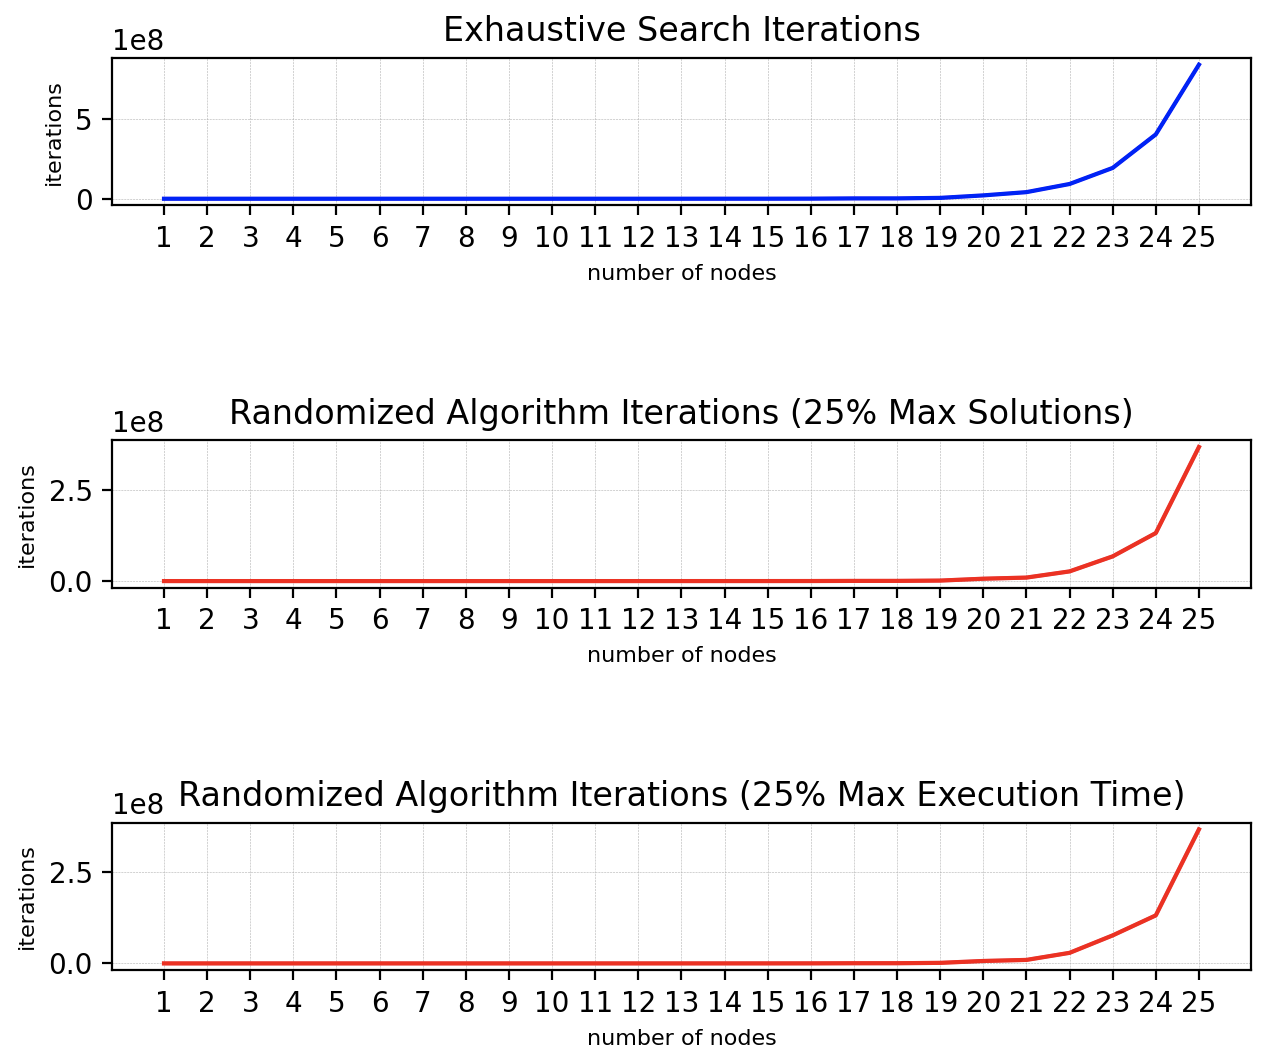
\includegraphics[width=0.9\columnwidth]{./figures/iterations_0.25.png}
    \caption{Iterations Number on the Exhaustive and Randomized Algorithms\label{iterations}}
    \label{fig: Iterations on the Exhaustive and Randomized Algorithms}
\end{figure}

Finally, comparing both algorithms regarding the iterations number [\ref{iterations}], we can see that, using both the \textbf{-s} and \textbf{-t} parameters, the number of iterations was approximately half of the iterations of the exhaustive search. This can be the supposed results, but can also be a bug when computing the iterations of the algorithm.

\begin{figure}[!htbp]
    \centering
    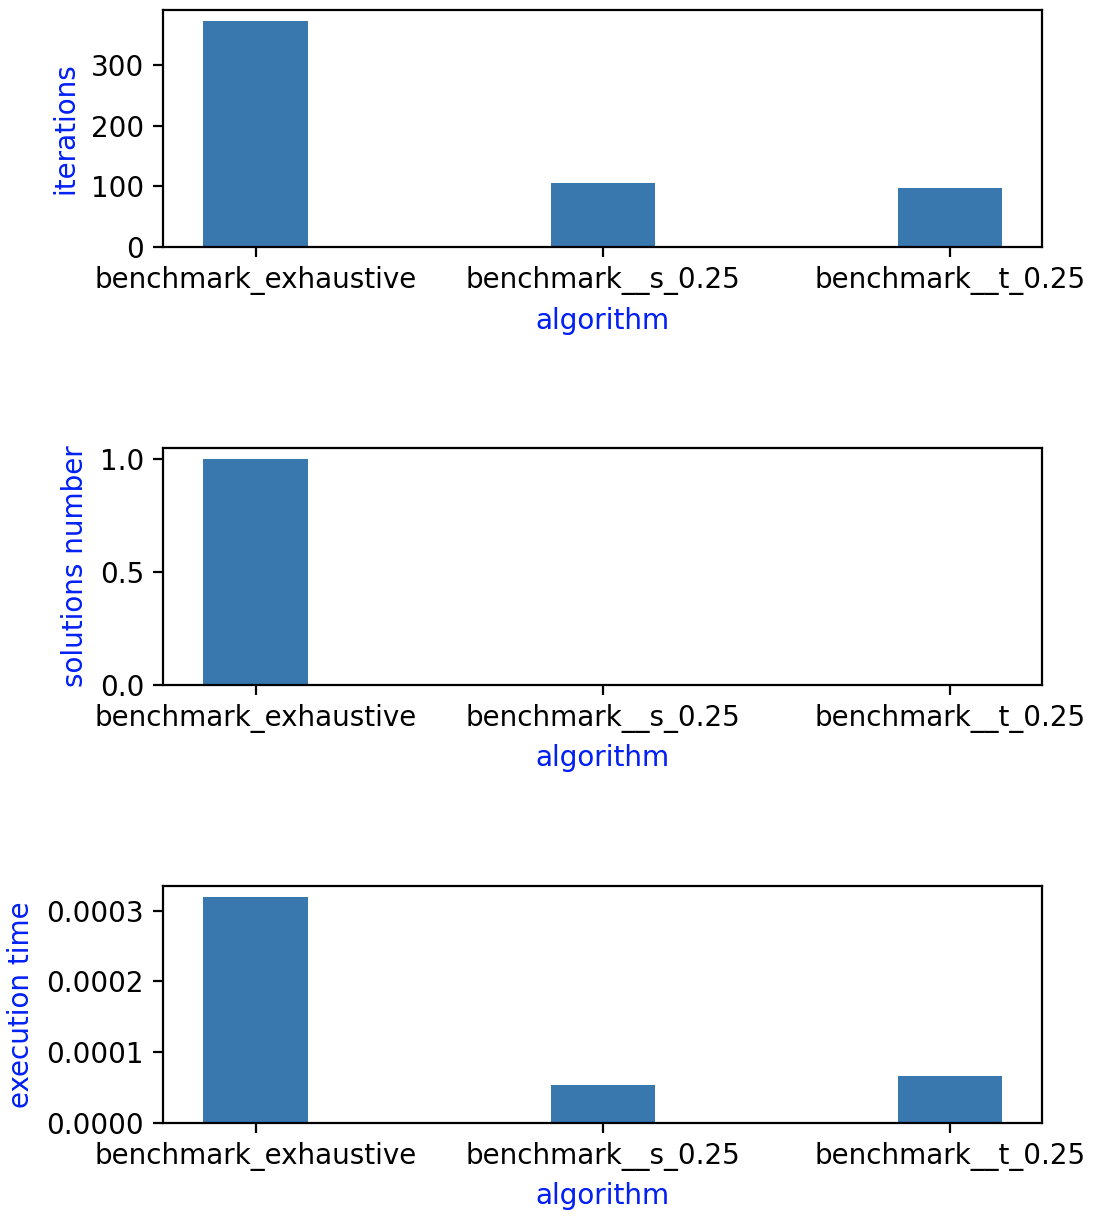
\includegraphics[width=0.8\columnwidth]{./figures/benchmark.png}
    \caption{Comparison between Exhaustive Search and Randomized Algorithms using the \textit{SWtinyEWD.txt} file\label{benchmark}}
    \label{fig: Comparison between Exhaustive Search and Randomized Algorithms using the SWtinyEWD.txt file}
\end{figure}

Using the benchmark file to compute the above-mentioned parameters [\ref{benchmark}], the results are as expected. Due to the graphs' size being small, regarding the number of solutions found, we can see that, as probably the subset that contained all nodes was not computed, the number of solutions the randomized algorithm returned was zero.

\section{Conclusion}

This assignment allowed for a better understanding of a randomized algorithm and its variations. Although the randomized algorithm performed better than the exhaustive one, regarding the iterations numbers, as well as execution time, the algorithm does not always return a solution, and when it does, most of the time it is not the optimal one. The randomized algorithm may be seen as a mid-term between the brute force method and the greedy one, both compared to the previous assignment.

\section{Future Work}

A feature that could be implemented is the ability of the algorithm to decide when  to  stop  testing  candidate solutions  of  a  certain  size  and  start  testing larger or smaller solutions. This feature, despite not being implemented in this solution, can be done as a future work of the project.

\begin{thebibliography}{9}

\bibitem{randomized_algorithms}
GeeksforGeeks. (2022, October 22). Randomized Algorithms. GeeksforGeeks. \url{https://www.geeksforgeeks.org/randomized-algorithms/}

\bibitem{random}
Python Software Foundation. (2001-2022). random — Generate pseudo-random numbers. 
\url{https://docs.python.org/3/library/random.html}

\end{thebibliography}


% use a field named url or \url{} for URLs
% Note: the \bibliographystyle is set automatically

\end{document}
